% Authors: Greg Westphal and Kathryn Huff
\documentclass[border=10pt]{standalone}
\usepackage{tikz}
\usetikzlibrary{arrows.meta}
\tikzset{%
  >={Latex[width=2mm,length=2mm]},
  % Specifications for style of nodes:
            base/.style = {rectangle, rounded corners, draw=black,
                           minimum width=3cm, minimum height=1cm,
                           text centered, font=\sffamily},
       bluebox/.style = {base, fill=gray!15}, %blue!30
       redbox/.style = {base, fill=white!30}, %red
       greenbox/.style = {base, fill=white!30}, %green
       process/.style = {base, minimum width=2.5cm, fill=gray!30, %orange!15
                           font=\ttfamily},
}
% Drawing part, node distance is 1.5 cm and every node
% is prefilled with white background
\begin{document}
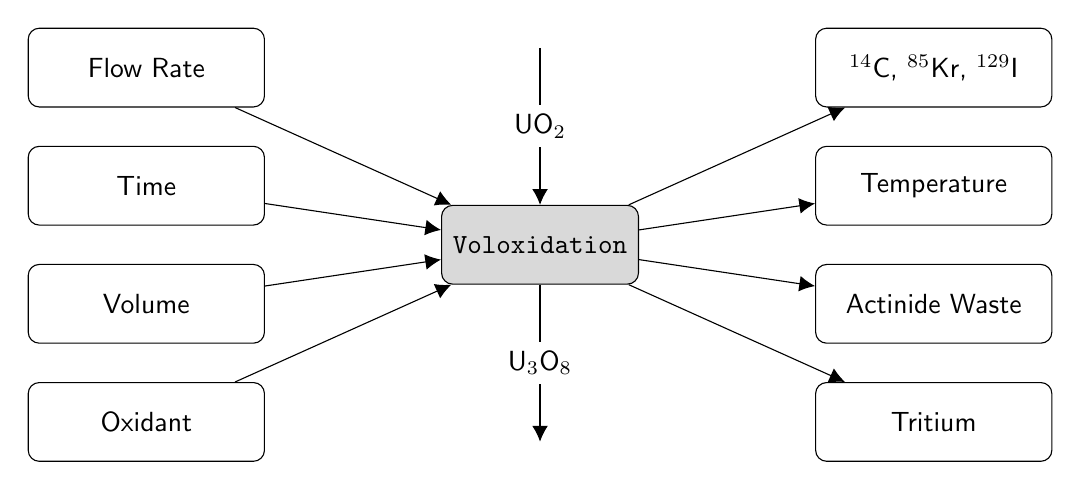
\begin{tikzpicture}[node distance=3cm,
    every node/.style={fill=white, font=\sffamily}, align=center]
  % Specification of nodes (position, etc.)
  
  \node (volox)				[process] {Voloxidation};
  \node (time)				[greenbox, left of=volox, xshift=-2cm, yshift=0.75cm] {Time};
  \node (vol)	 			[greenbox, left of=volox, xshift=-2cm, yshift=-0.75cm] {Volume};
  \node (flow)				[greenbox, left of=volox, xshift=-2cm, yshift=2.25cm] {Flow Rate};
  \node (oxidant)			[greenbox, left of=volox, xshift=-2cm, yshift=-2.25cm] {Oxidant};
  \node (temp)				[redbox, right of=volox, xshift=2cm, yshift=0.75cm] {Temperature};
  \node (gas) 				[redbox, right of=volox, xshift=2cm, yshift=2.25cm] {$^{14}$C, $^{85}$Kr, $^{129}$I}; 
  \node (actinide)			[redbox, right of=volox, xshift=2cm, yshift=-0.75cm] {Actinide Waste};
  \node (tritium)			[redbox, right of=volox, xshift=2cm, yshift=-2.25cm] {Tritium};
  
  \draw[->]					(volox)++(0,2.5) -- (volox) node[midway] {UO$_2$};
  \draw[->]					(volox) -- (tritium);
  \draw[->] 				(volox) -- (gas);
  \draw[->]					(volox) -- (actinide);
  \draw[->]					(time) -- (volox);
  \draw[->]					(volox) -- (temp);
  \draw[->]					(oxidant) -- (volox);
  \draw[->]					(volox) -- ++(0,-2.5) node[midway] {U$_3$O$_8$};
  \draw[->]					(vol) -- (volox);
  \draw[->]					(flow) -- (volox);
  \end{tikzpicture}
\end{document}